\documentclass[11pt, letterpaper]{article}

% ----- PACKAGES -----
\usepackage[utf8]{inputenc}
\usepackage[T1]{fontenc}
\usepackage{OldStandard}
\usepackage{anyfontsize}
\usepackage{geometry}
\geometry{margin=1in}
\usepackage{titlesec}
\usepackage{array}
\usepackage{enumitem}
\usepackage{xcolor}
\usepackage[most]{tcolorbox}
\usepackage{hyperref}
\usepackage{booktabs}
\usepackage{tabularx}
\usepackage{makecell}
\usepackage{graphicx}
\usepackage{caption}
\usepackage{float}

% ----- HYPERLINK SETUP -----
\hypersetup{
    colorlinks=true,
    linkcolor=black,
    filecolor=magenta,
    urlcolor=blue,
    pdftitle={SafeSurveil-AIxBio Research Report}
}

% ----- HEADING SIZES -----
\titleformat{\section}{\fontsize{14}{17}\bfseries}{\thesection.}{0.5em}{}
\titleformat{\subsection}{\fontsize{14}{17}\bfseries}{}{0em}{}

% ----- CUSTOM COLORS -----
\definecolor{boxbg}{HTML}{FFF2CC}
\definecolor{deepnavy}{HTML}{071323}
\definecolor{slate}{HTML}{31445B}
\definecolor{softblue}{HTML}{EAF2FA}
\definecolor{softgreen}{HTML}{EAF8F0}
\definecolor{softamber}{HTML}{FFF4DA}
\definecolor{softred}{HTML}{FFF0EE}
\definecolor{rulegray}{HTML}{CAD5E2}

\newcommand{\project}{SafeSurveil-AIxBio}
\newcommand{\codepending}{\textit{Public repository URL to be inserted after visibility update.}}
\newcommand{\pcite}[1]{[\ref{#1}]}

\setlength{\parskip}{0.45em}
\setlength{\parindent}{0em}
\emergencystretch=3em
\sloppy

\begin{document}

% ==========================================
% TITLE & HEADER BLOCK
% ==========================================
\noindent\rule{\textwidth}{1.5pt} \par
\vspace{0.4cm}
\begin{center}
    {\fontsize{20}{24}\selectfont \textbf{\project: Evidence-Gated Genomic AMR Triage with Grounded AI Copilots}\footnotemark}
\end{center}
\vspace{0.1cm}
\noindent\rule{\textwidth}{0.5pt} \par
\vspace{0.65cm}

\footnotetext{Research conducted at the \href{https://apartresearch.com/sprints/aixbio-hackathon-2026-04-24-to-2026-04-26}{AIxBio Hackathon}, April 2026}

% ----- AUTHOR BLOCK -----
\begin{center}
\begin{tabular}{@{}c@{}}
\textbf{M. Rishyanth Reddy, V. Eswar} \\
Vignan's Lara Institute of Technology \& Science \\
Vadlamudi, Andhra Pradesh, India \\
\href{mailto:rishyanthreddy101@gmail.com}{rishyanthreddy101@gmail.com} \\
\href{mailto:eswarvajja16@gmail.com}{eswarvajja16@gmail.com} \\[0.35cm]
\textbf{G. Akash Reddy} \\
Glocal University \\
Saharanpur, Uttar Pradesh, India \\
\href{mailto:gade.akash3456@gmail.com}{gade.akash3456@gmail.com}
\end{tabular}
\end{center}
\vspace{0.2cm}

\begin{center}
    \textbf{With} \\
    Apart Research
\end{center}
\vspace{0.4cm}

% ==========================================
% ABSTRACT
% ==========================================
\begin{center}
    \textbf{\fontsize{14}{17}\selectfont Abstract}
\end{center}
\vspace{0.1cm}

\begin{center}
\begin{minipage}{0.78\textwidth}
\noindent\textit{Rapid genomic surveillance can shorten the path from antimicrobial-resistance (AMR) signal detection to analyst review, but AI-assisted workflows are difficult to trust when evidence provenance, model limits, and generated explanations are separated across tools. We present \project, a defensive prototype for \textit{E. coli}--tetracycline triage that couples live public-data retrieval and local AMR evidence generation with an auditable operator interface. The system ingests a live-retrieved FASTA, records source provenance and artifact hashes, normalizes AMRFinderPlus mechanisms, estimates novelty and baseline phenotype risk, and produces an actionability-constrained triage decision. Its main contribution is a runtime trust layer rather than a new clinical predictor: generated copilot and semantic-UI outputs are treated as sidecars and accepted only after identity, citation, numeric, queue-context, and policy checks against the persisted decision object. \project{} also builds a deterministic biological reasoning trace, typed evidence graph, execution-gate verdict, and V2 audit page. In the final proof run, a frontend-submitted live job completed with OpenRouter live output, Thesys rendered output, \texttt{gate=allow}, full consistency checks, a 54-node/101-edge evidence graph, and a 26/0/0 pass/warn/fail curl matrix. The prototype is not clinically validated; it demonstrates how genomic AI triage can be made inspectable, bounded, and submission-auditable.}
\end{minipage}
\end{center}
\vspace{0.45cm}

% ==========================================
% MAIN BODY SECTIONS
% ==========================================
\section{Introduction}

Antimicrobial resistance is a biosecurity and public-health problem because the same signals that matter for routine stewardship--resistance genes, phenotype predictions, mobile elements, novelty, and surveillance provenance--also determine how quickly an analyst can identify a case that deserves attention. Whole-genome sequencing (WGS) has expanded what can be detected in AMR surveillance, but the literature repeatedly cautions that database choice, phenotype-genotype discordance, and standardization affect interpretation [\ref{boolchandani2019}, \ref{hendriksen2019}, \ref{mahfouz2020}]. At the same time, machine-learning systems for infectious-disease decision support remain difficult to deploy safely because many are evaluated primarily by predictive performance rather than workflow impact, external validation, or interpretability [\ref{peiffer2020}, \ref{ardila2024}, \ref{ardila2025}].

\project{} addresses a narrow but important failure mode: AI can make AMR triage look more certain than the evidence allows. The prototype therefore treats generated language and rendered UI as sidecars. The authoritative objects are persisted decisions, evidence artifacts, provenance records, and verifier outputs. In a hackathon setting, this lets us demonstrate a practical theory of change: a local analyst can inspect a genomic AMR case rapidly while seeing why the system allows, reviews, or blocks downstream action.

\textbf{Our main contributions are:}
\begin{enumerate}
    \item A live-backed AMR triage workflow connecting public-data retrieval, local AMR tooling, persisted decision objects, grounded copilot generation, and renderer-safe frontend presentation.
    \item A visible execution gate that checks identity, citations, numeric consistency, policy alignment, evidence coverage, provider mode, and audit fingerprints before generated content is trusted.
    \item A deterministic reasoning trace and evidence graph that convert the case into inspectable biological and operational evidence rather than a black-box recommendation.
    \item A V2 evaluation page and reproducible curl/browser proof bundle that make hackathon acceptance claims auditable rather than anecdotal.
\end{enumerate}

\section{Related Work}

\textbf{Genomic AMR surveillance.} WGS and metagenomic approaches are increasingly important for AMR detection, outbreak investigation, food-chain surveillance, and One Health monitoring [\ref{boolchandani2019}, \ref{oniciuc2018}, \ref{collineau2019}]. Reviews of AMR bioinformatics tools emphasize that resources such as AMRFinder, CARD, ResFinder, ARG-ANNOT, and related databases differ in input assumptions, search strategy, marker coverage, and sensitivity/specificity tradeoffs [\ref{hendriksen2019}, \ref{mahfouz2020}]. This directly shaped our design: the UI shows mechanistic evidence, raw artifact IDs, support levels, and caveats instead of presenting gene detection as a final clinical answer.

\textbf{ML for AMR and stewardship.} Systematic reviews find promising performance for ML models that predict AMR from WGS, AST, clinical, or stewardship data, with common algorithms including random forests, gradient boosting, logistic regression, and XGBoost [\ref{ardila2024}, \ref{ardila2025}, \ref{pinto2024}]. However, these reviews also identify barriers: retrospective designs, nonstandard preprocessing, limited prospective clinical validation, and high-income-setting bias \pcite{peiffer2020}. \project{} therefore does not claim broad predictive superiority. Its predictive baseline is deliberately disclosed as fixture-trained; the novelty is how predictions are constrained, explained, and audited in a live workflow.

\textbf{LLMs and clinical safety.} Recent reviews of LLMs in healthcare and antibiotic guidance report potential utility but consistent concerns around hallucination, guideline mismatch, privacy, patient-safety risk, and the need for human oversight [\ref{park2024}, \ref{antonie2025}, \ref{algain2025}]. Retrieval-augmented generation (RAG) is a promising grounding strategy, but healthcare RAG still lacks standardized evaluation and ethical reporting practices \pcite{amugongo2025}. In response, \project{} validates generated citations against the built copilot context, rejects fabricated numbers, labels cached/fallback/live modes, and refuses out-of-bound requests.

\textbf{Explainability, evidence graphs, and biological reasoning.} XAI reviews argue that clinical decision support requires explanations that are meaningful to end users, not only post-hoc feature scores [\ref{antoniadi2021}, \ref{xu2023}]. Biomedical knowledge graphs are widely explored for integrating heterogeneous evidence, but translation to clinical practice remains challenging [\ref{budhdeo2023}, \ref{rajabi2022}]. Recent BioReason work similarly emphasizes structured biological reasoning traces from genomic or protein context [\ref{fallahpour2025}, \ref{fallahpour2026}]. \project{} borrows that interpretability spirit without claiming to be a BioReason model: it deterministically assembles a reasoning trace from persisted AMR evidence, novelty, QC, actionability, and triage.

\section{Methods}

\subsection*{System Scope and Claim Boundary}

The implemented scope is intentionally narrow: \textit{E. coli} plus tetracycline, local-first execution, live integration paths where configured, and a fixture-trained smoke predictive baseline. The system is not a diagnostic, not a treatment recommender, and not validated for broad AMR deployment. It is a defensive surveillance decision-support prototype for analyst review.

\subsection*{Pipeline}

\begin{figure}[H]
\centering
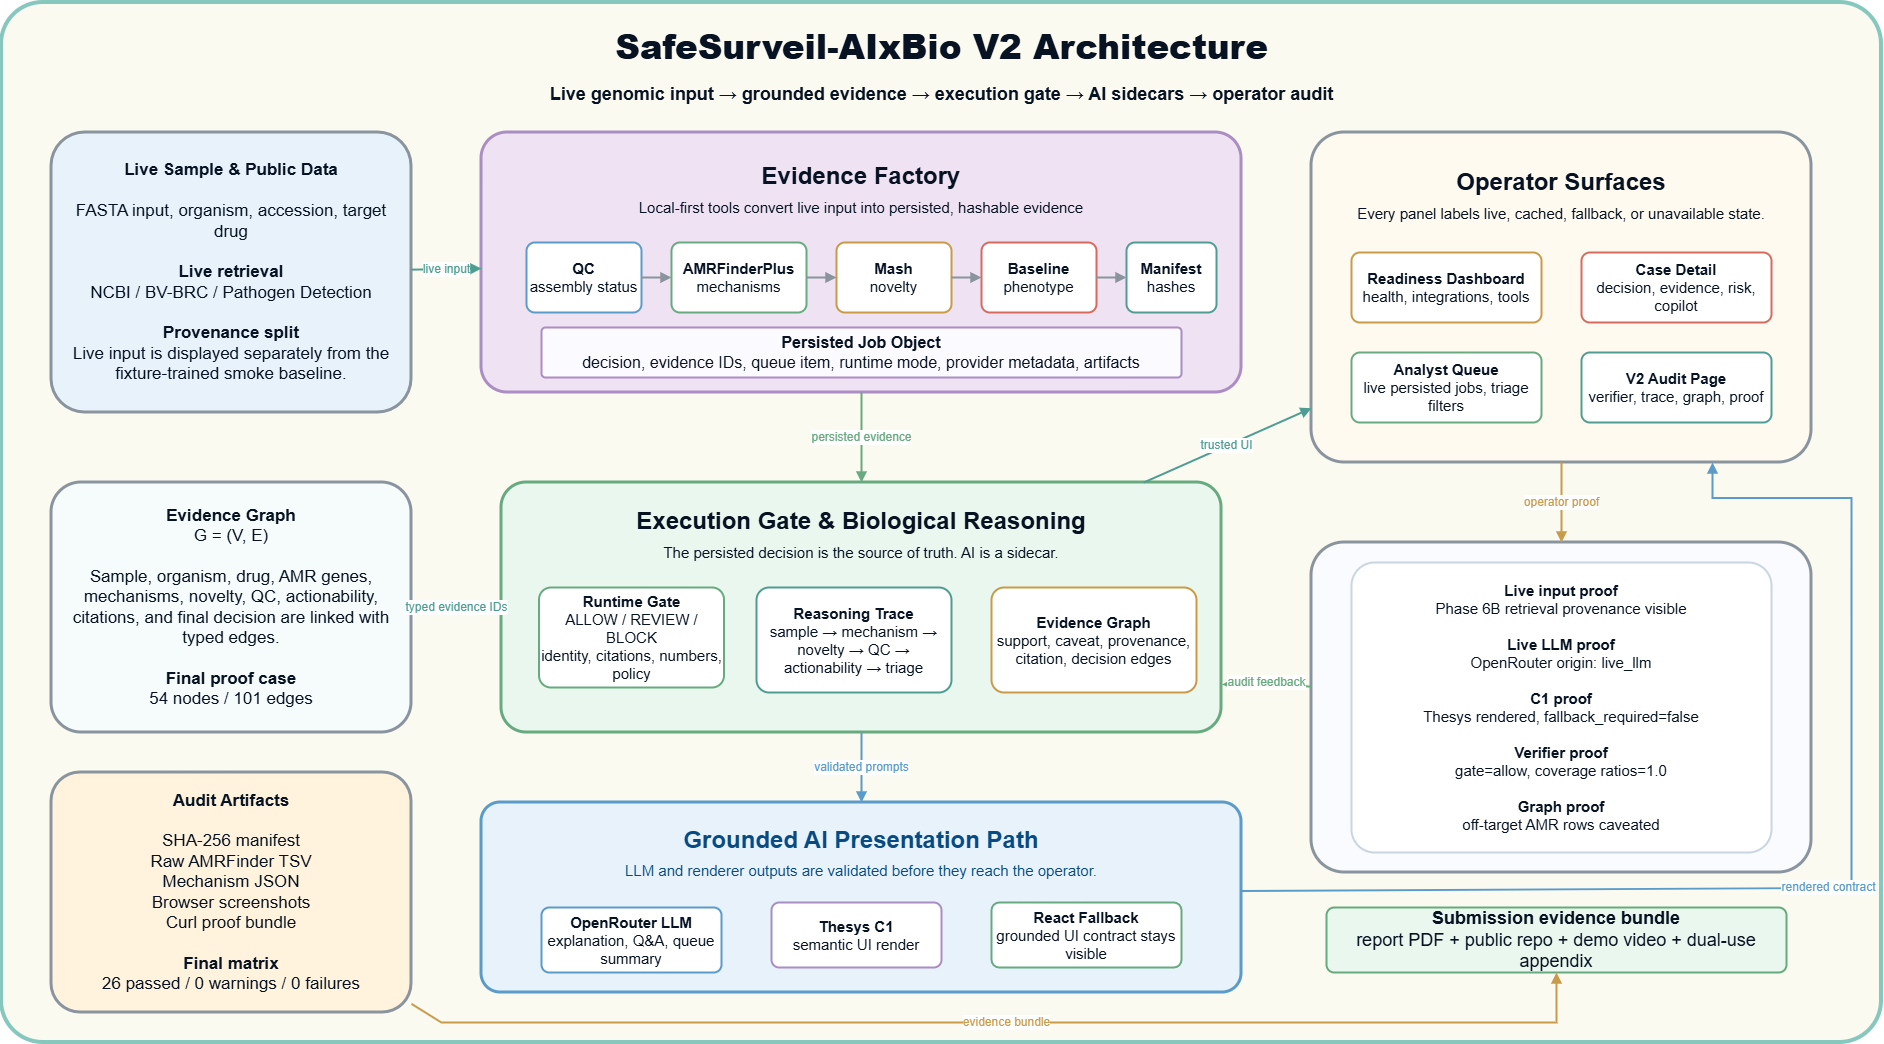
\includegraphics[width=\textwidth]{../figures/safesurveil_architecture_report.png}
\caption{SafeSurveil-AIxBio V2 architecture. Live genomic input is converted into persisted evidence artifacts, checked by an execution gate and deterministic reasoning layer, then exposed through validated AI sidecars and operator-facing audit surfaces.}
\label{fig:architecture}
\end{figure}

\subsection*{Execution Gate and Grounding Checks}

The verifier treats the persisted decision object as the source of truth. It checks whether generated and rendered objects preserve job identity, sample identity, target drug, triage fields, numeric values, cited evidence IDs, queue context, policy alignment, and artifact coverage. It also records provider-call metadata so deterministic verifier routes do not accidentally trigger live LLM or renderer calls. The gate returns \texttt{allow}, \texttt{review}, or \texttt{block}; the frontend displays that result upstream of generated copilot text.

\subsection*{Reasoning Trace and Evidence Graph}

The reasoning trace is not chain-of-thought from the LLM. It is a deterministic, auditable sequence over known case components: sample context, AMR mechanism evidence, phenotype prediction, novelty, QC limits, actionability, triage, and final operator guidance. The evidence graph builds nodes for sample, organism, drug, genes, mechanism classes, artifacts, novelty, QC, actionability, rationale codes, copilot citations, and final decision. Edges are typed as support, caveat, provenance, citation, or decision linkage. Off-target or weak AMR mechanisms are caveated rather than shown as supporting target-drug actionability.

\section{Results}

\subsection*{Implementation Outcome}

The hackathon build produced a working backend, frontend, and trust-layer bundle. The final live proof used frontend-created job \texttt{job\_20260425201118267288} for sample \texttt{frontend\_live\_final\_20260425201057}. The submitted FASTA path came from the Phase 6B live-retrieval flow with source context \texttt{agricultural\_surveillance\_proxy}. Runtime health reported live evidence mode, live LLM mode, and no live blockers.

\begin{table}[H]
\centering
\small
\begin{tabularx}{\textwidth}{p{0.25\textwidth}p{0.22\textwidth}X}
\toprule
\textbf{Check} & \textbf{Observed Result} & \textbf{Interpretation} \\
\midrule
Backend regression suite & 204 passed, 30 deselected & Non-live contract and service tests passed before closure. \\
Explicit live suite & 30 passed, 204 deselected & Live integration tests passed separately from deterministic tests. \\
Frontend typecheck/build & Passed & React/TypeScript build was production-buildable; only existing large-chunk warning remained. \\
V2 curl matrix & 26 passed, 0 warnings, 0 failures & Backend, provider, proxy, verifier, trace, graph, and audit checks passed for the selected job. \\
Provider proof & OpenRouter \texttt{live\_llm}; Thesys C1 \texttt{rendered} & Generated sidecars were exercised live in the final proof. \\
Execution gate & \texttt{allow}; 0 failed, 0 warning checks & The selected case passed identity, evidence, numeric, citation, and policy checks. \\
Evidence graph & 54 nodes, 101 edges, completeness 1.0 & The case was represented as an inspectable evidence graph. \\
\bottomrule
\end{tabularx}
\caption{Final recorded hackathon proof bundle. These are engineering verification results, not clinical validation results.}
\label{tab:proof}
\end{table}

\subsection*{What the Demo Shows}

The final operator flow starts at runtime readiness, submits or selects a live-backed job, opens the analyst queue, inspects the case detail screen, reviews mechanistic evidence and artifact hashes, checks novelty and risk decomposition, asks grounded copilot questions, renders semantic UI through Thesys C1 or React fallback, and closes on the V2 audit page. The key result is that every generated or visual sidecar is subordinate to the persisted decision and evidence artifacts. If a provider fails, cached/fallback labels are visible; if grounding is weak, refusal and warnings are surfaced instead of being hidden.

\section{Discussion and Limitations}

\project{} demonstrates that a biosecurity-facing AMR triage tool can be designed around visible constraints rather than invisible model authority. This matters because both AMR surveillance and healthcare AI literatures point to the same adoption barrier: promising models are not enough when users cannot see provenance, limitations, failure modes, or whether generated text is grounded [\ref{peiffer2020}, \ref{antoniadi2021}, \ref{park2024}]. The execution gate, reasoning trace, and evidence graph are therefore not decorative. They are part of the safety interface.

\subsection*{Limitations}

The current prototype is not clinically validated. It focuses on a narrow \textit{E. coli}--tetracycline scenario and uses a fixture-trained smoke baseline for the first predictive layer. It does not establish sensitivity, specificity, calibration, robustness across pathogens, or prospective clinical utility. Live input provenance was demonstrated, but large-scale public-data evaluation is reserved for V3. The LLM and Thesys integrations are live sidecars, but provider outputs remain bounded by validation and should not be treated as independent scientific evidence.

\subsection*{Future Work}

The next research-grade version should add multi-sample public AMR snapshots, leakage-controlled train/test splits, random-versus-lineage split comparison, calibrated baselines, ablations for mechanism/novelty/QC/gate components, unsafe-ACT-rate metrics, external validation, and reproducible statistical reporting. A practitioner study would strengthen the work, but a computational-only Q1-reach path is still plausible if the evaluation is broad, rigorous, and honest about dual-use boundaries.

\section{Conclusion}

\project{} is a hackathon-grade proof that AI-assisted genomic AMR triage can be built around evidence governance rather than model mystique. The system connects live AMR evidence, grounded generation, renderer-safe presentation, and a visible execution gate into one analyst workflow. Its most important result is not that it predicts resistance better than existing methods; it shows how a defensive biosecurity tool can make provenance, uncertainty, citations, and generated-language boundaries visible by default.

\section*{Code and Data}

\begin{itemize}[label=-]
    \item \textbf{Code repository:} \codepending
    \item \textbf{Data and artifacts:} The report uses local hackathon artifacts, public-data retrieval paths, generated AMRFinderPlus output, artifact manifests, and V2 proof summaries. Credentials and local \texttt{.env} files are excluded from release.
    \item \textbf{Demo video:} To be recorded and linked by the authors before submission.
\end{itemize}

\section*{Author Contributions}

M. Rishyanth Reddy led the project concept, implementation workflow, integration testing, frontend review, and report direction. V. Eswar and G. Akash Reddy contributed to project development, validation, and report preparation. Apart Research organized the AIxBio Hackathon and provided the submission template/event context.

\section*{References}

\begin{enumerate}[leftmargin=*]
    \item \label{boolchandani2019} Boolchandani, M. et al. (2019). Sequencing-based methods and resources to study antimicrobial resistance. \textit{Nature Reviews Genetics}. \href{https://consensus.app/papers/details/435fbf72968c509e9a860a6c87d62175/?utm_source=unknown}{View on Consensus}.
    \item \label{hendriksen2019} Hendriksen, R. et al. (2019). Using Genomics to Track Global Antimicrobial Resistance. \textit{Frontiers in Public Health}. \href{https://consensus.app/papers/details/63ca2e3f2d9351809e2a67a5125cb606/?utm_source=unknown}{View on Consensus}.
    \item \label{oniciuc2018} Oniciuc, E.-A. et al. (2018). The Present and Future of Whole Genome Sequencing and Whole Metagenome Sequencing for Surveillance of AMR. \textit{Genes}. \href{https://consensus.app/papers/details/05f276609d5255abb0f4d6afd48851b5/?utm_source=unknown}{View on Consensus}.
    \item \label{collineau2019} Collineau, L. et al. (2019). Integrating Whole-Genome Sequencing Data Into Quantitative Risk Assessment of Foodborne AMR. \textit{Frontiers in Microbiology}. \href{https://consensus.app/papers/details/933edec6750e535fa356054fabf4c17f/?utm_source=unknown}{View on Consensus}.
    \item \label{mahfouz2020} Mahfouz, N. et al. (2020). Large-scale assessment of antimicrobial resistance marker databases for genetic phenotype prediction. \textit{Journal of Antimicrobial Chemotherapy}. \href{https://consensus.app/papers/details/656f5d8c9ae5558e8d3abbb81aaeff63/?utm_source=unknown}{View on Consensus}.
    \item \label{su2018} Su, M. et al. (2018). Genome-Based Prediction of Bacterial Antibiotic Resistance. \textit{Journal of Clinical Microbiology}. \href{https://consensus.app/papers/details/06e5710440fa5f90825a2a79cd48ffc6/?utm_source=unknown}{View on Consensus}.
    \item \label{peiffer2020} Peiffer-Smadja, N. et al. (2020). Machine learning for clinical decision support in infectious diseases. \textit{Clinical Microbiology and Infection}. \href{https://consensus.app/papers/details/72fce91a95125f52a36c655e1406d4e9/?utm_source=unknown}{View on Consensus}.
    \item \label{ardila2024} Ardila, C. M. et al. (2024). Integrating whole genome sequencing and machine learning for predicting antimicrobial resistance in critical pathogens. \textit{PeerJ}. \href{https://consensus.app/papers/details/dd18acba2ab1532982dc97a67e2ec704/?utm_source=unknown}{View on Consensus}.
    \item \label{ardila2025} Ardila, C. et al. (2025). Machine learning for predicting antimicrobial resistance in critical and high-priority pathogens. \textit{PLOS One}. \href{https://consensus.app/papers/details/3c1bc3a411a65ac5abfd9bf035c15316/?utm_source=unknown}{View on Consensus}.
    \item \label{pinto2024} Pinto-de-Sa, R. et al. (2024). Brave New World of Artificial Intelligence: Its Use in Antimicrobial Stewardship--A Systematic Review. \textit{Antibiotics}. \href{https://consensus.app/papers/details/4b1d1024b494588cb81b97afa00e80a6/?utm_source=unknown}{View on Consensus}.
    \item \label{algain2025} AlGain, S. et al. (2025). Can we rely on artificial intelligence to guide antimicrobial therapy? \textit{Antimicrobial Stewardship \& Healthcare Epidemiology}. \href{https://consensus.app/papers/details/a9e8e10b1f805a0a888faef3767e2ff2/?utm_source=unknown}{View on Consensus}.
    \item \label{antonie2025} Antonie, N.-I. et al. (2025). The Role of ChatGPT and AI Chatbots in Optimizing Antibiotic Therapy. \textit{Antibiotics}. \href{https://consensus.app/papers/details/d66b7ce37dd2588c8418dcb1c8a6895b/?utm_source=unknown}{View on Consensus}.
    \item \label{park2024} Park, Y.-J. et al. (2024). Assessing the research landscape and clinical utility of large language models. \textit{BMC Medical Informatics and Decision Making}. \href{https://consensus.app/papers/details/89c0222087fa5c39b88eb06a4d71df0d/?utm_source=unknown}{View on Consensus}.
    \item \label{amugongo2025} Amugongo, L. M. et al. (2025). Retrieval augmented generation for large language models in healthcare. \textit{PLOS Digital Health}. \href{https://consensus.app/papers/details/9d1904c2383e5dcc954c87f5ad10a66f/?utm_source=unknown}{View on Consensus}.
    \item \label{antoniadi2021} Antoniadi, A. et al. (2021). Current Challenges and Future Opportunities for XAI in ML-Based Clinical Decision Support Systems. \textit{Applied Sciences}. \href{https://consensus.app/papers/details/d3f76f92a3575f96bec1e0c22c80a9f3/?utm_source=unknown}{View on Consensus}.
    \item \label{xu2023} Xu, Q. et al. (2023). Interpretability of Clinical Decision Support Systems Based on Artificial Intelligence. \textit{Journal of Healthcare Engineering}. \href{https://consensus.app/papers/details/c3536b48507e527aa7049dddaa55ef84/?utm_source=unknown}{View on Consensus}.
    \item \label{budhdeo2023} Budhdeo, S. et al. (2023). Scoping review of knowledge graph applications in biomedical and healthcare sciences. \textit{Wellcome Open Research}. \href{https://consensus.app/papers/details/9c5d9984fda35ff3a299fa0a726f1607/?utm_source=unknown}{View on Consensus}.
    \item \label{rajabi2022} Rajabi, E. and Etminani, K. (2022). Knowledge-graph-based explainable AI: A systematic review. \textit{Journal of Information Science}. \href{https://consensus.app/papers/details/affdd66df0055d2596d7f155c3857fc4/?utm_source=unknown}{View on Consensus}.
    \item \label{undheim2024} Undheim, T. (2024). The whack-a-mole governance challenge for AI-enabled synthetic biology. \textit{Frontiers in Bioengineering and Biotechnology}. \href{https://consensus.app/papers/details/d13cdf4c37085be28493ea131ec8a1ca/?utm_source=unknown}{View on Consensus}.
    \item \label{elgabry2024} Elgabry, M. et al. (2024). Cyber-biological convergence: a systematic review and future outlook. \textit{Frontiers in Bioengineering and Biotechnology}. \href{https://consensus.app/papers/details/f773095e6925525a83eddd97ecb678de/?utm_source=unknown}{View on Consensus}.
    \item \label{fallahpour2025} Fallahpour, A. et al. (2025). BioReason: Incentivizing Multimodal Biological Reasoning within a DNA-LLM Model. \textit{arXiv}. \href{https://arxiv.org/abs/2505.23579}{View on arXiv}.
    \item \label{fallahpour2026} Fallahpour, A. et al. (2026). BioReason-Pro: Advancing Protein Function Prediction with Multimodal Biological Reasoning. \textit{BioRxiv / Arc Institute}. \href{https://arcinstitute.org/news/bioreason-pro}{View source}.
\end{enumerate}

\section*{Appendix: Limitations and Dual-Use Considerations}

\textbf{False positives and false negatives.} A gene call, similarity score, or phenotype probability can be wrong or incomplete. The prototype mitigates this by surfacing evidence IDs, support levels, QC warnings, and lab-confirmation next steps, but it does not eliminate biological uncertainty.

\textbf{Scalability constraints.} The current implementation is local-first and scoped to a narrow demo case. It has not been benchmarked across diverse organisms, drugs, sequencing technologies, or surveillance settings.

\textbf{Dual-use risks.} AMR surveillance tools can be misused if they help optimize harmful biological choices, identify resistance patterns for misuse, or make uncertain genomic signals appear operationally decisive. \project{} reduces but does not remove this risk by limiting outputs to defensive triage, avoiding autonomous action, preserving uncertainty, and treating generated text as non-authoritative.

\textbf{Responsible disclosure.} No new biological vulnerability or undisclosed pathogen finding was discovered during this work. If future versions identify actionable public-health or biosecurity concerns, disclosure should occur through institutional biosafety, public-health, or responsible-reporting channels before public release.

\textbf{Ethical posture.} The system is intended for defensive surveillance, analyst review, and safer decision support. It should not be used for clinical treatment, autonomous containment decisions, or high-consequence action without validated laboratory confirmation and appropriate expert oversight.

\section*{LLM Usage Statement}

LLM assistance was used during software development, code review, literature orientation, and report drafting. All reported implementation results, test counts, provider-proof states, and safety claims were checked against repository artifacts, acceptance matrices, or cited sources. Generated language was edited to preserve the authors' claim boundaries and to avoid overstating clinical validity.

\end{document}
